\subsection{ANYmal PPO-TV}
Thirty training seeds per setting. Bands are one sample SD across policy means, not confidence intervals. Ordinary standard is fixed; the best complete parameter is selected ex post separately per axis. 7/7 declared TV caps have full 30-seed suites; 29,491,200 native transitions per policy. Competence not certified by returns/completion.
\begin{figure}[p]\centering
\begin{subfigure}{0.48\textwidth}\centering
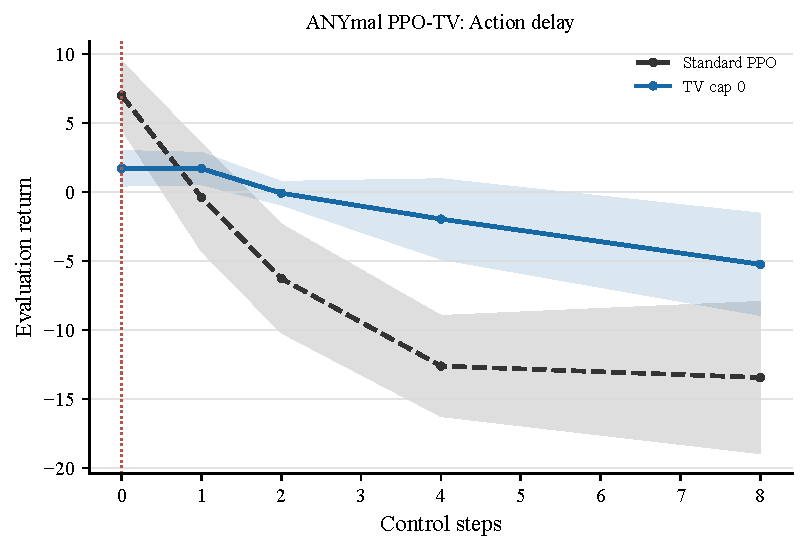
\includegraphics[width=\linewidth]{plots/anymal_ppo_tv30/action_delay.pdf}
\caption{Action delay}
\end{subfigure}\hfill
\begin{subfigure}{0.48\textwidth}\centering
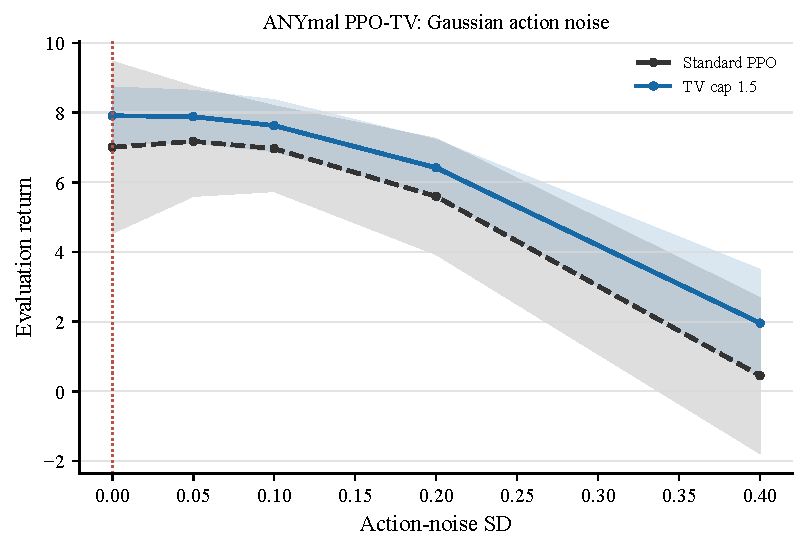
\includegraphics[width=\linewidth]{plots/anymal_ppo_tv30/action_noise.pdf}
\caption{Gaussian action noise}
\end{subfigure}\par\medskip
\begin{subfigure}{0.48\textwidth}\centering
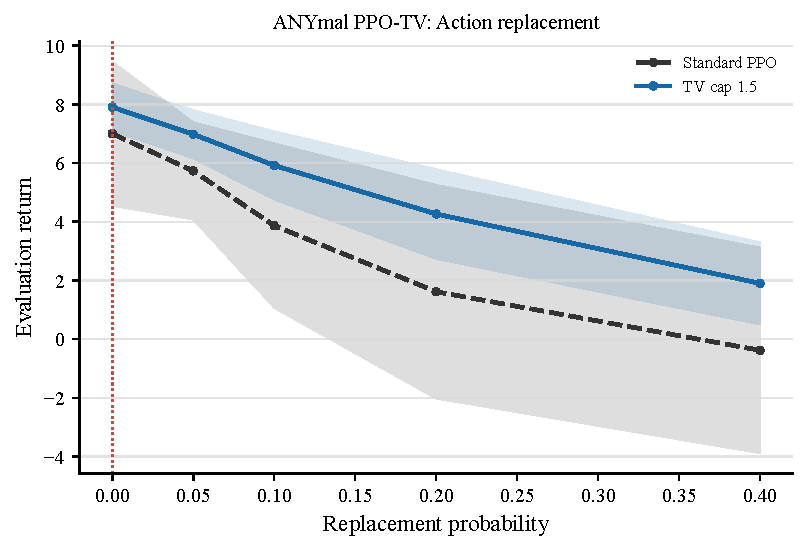
\includegraphics[width=\linewidth]{plots/anymal_ppo_tv30/action_replacement.pdf}
\caption{Action replacement}
\end{subfigure}\hfill
\begin{subfigure}{0.48\textwidth}\centering
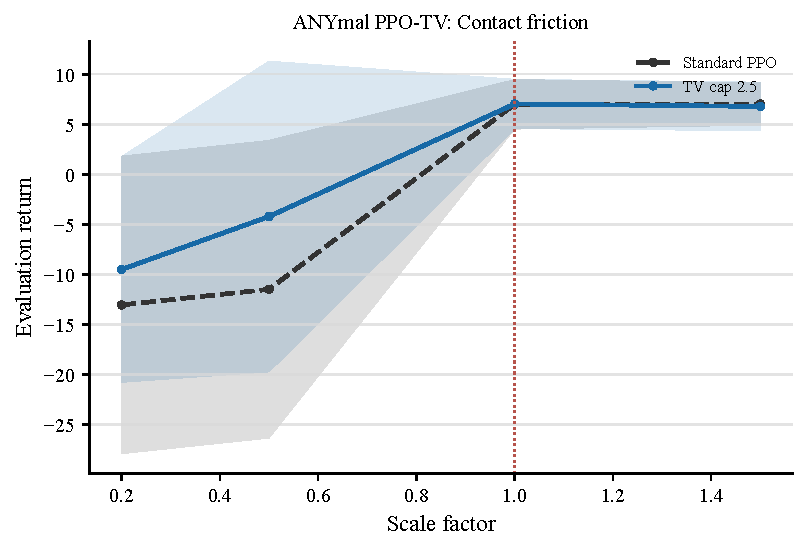
\includegraphics[width=\linewidth]{plots/anymal_ppo_tv30/contact_friction.pdf}
\caption{Contact friction}
\end{subfigure}\par\medskip
\caption{ANYmal PPO-TV. Mean and sample SD across 30 training seeds; ex-post selection.}
\end{figure}
\begin{figure}[p]\centering
\begin{subfigure}{0.48\textwidth}\centering
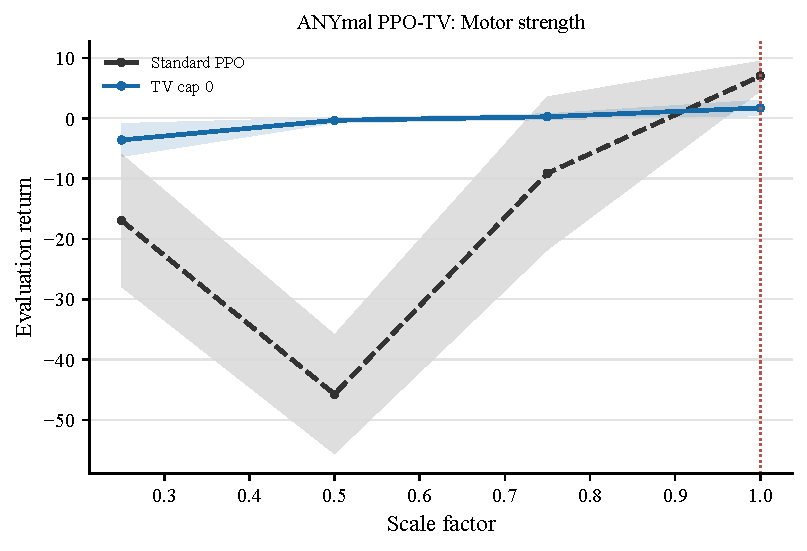
\includegraphics[width=\linewidth]{plots/anymal_ppo_tv30/motor_strength.pdf}
\caption{Motor strength}
\end{subfigure}\hfill
\begin{subfigure}{0.48\textwidth}\centering
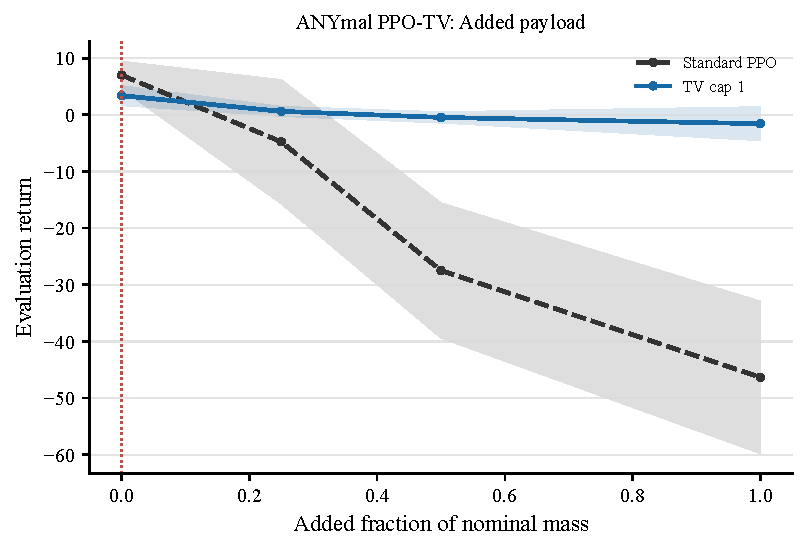
\includegraphics[width=\linewidth]{plots/anymal_ppo_tv30/payload_fraction.pdf}
\caption{Added payload}
\end{subfigure}\par\medskip
\caption{ANYmal PPO-TV. Mean and sample SD across 30 training seeds; ex-post selection.}
\end{figure}
\subsection{Ant PPO-TV}
Thirty training seeds per setting. Bands are one sample SD across policy means, not confidence intervals. Ordinary standard is fixed; the best complete parameter is selected ex post separately per axis. 1/6 declared TV caps have full 30-seed suites; 32,768,000 native transitions per policy. Competence not certified by returns/completion.
\begin{figure}[p]\centering
\begin{subfigure}{0.48\textwidth}\centering
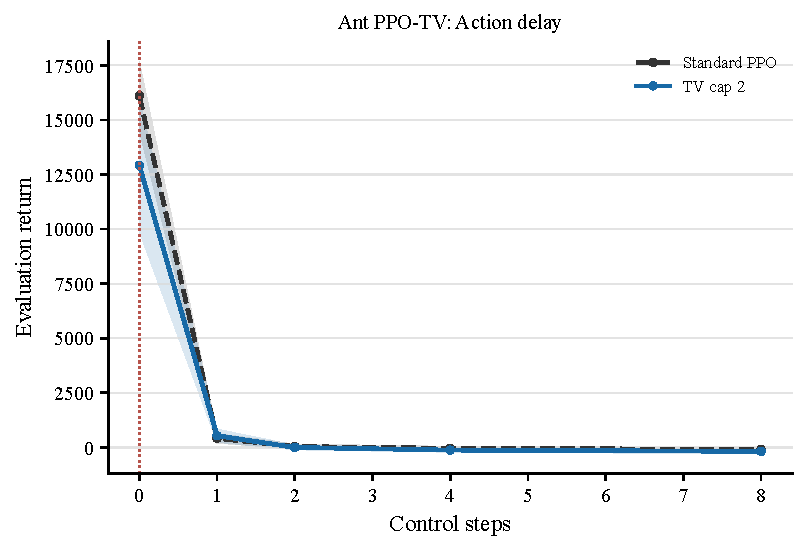
\includegraphics[width=\linewidth]{plots/ant_ppo_tv30/action_delay.pdf}
\caption{Action delay}
\end{subfigure}\hfill
\begin{subfigure}{0.48\textwidth}\centering
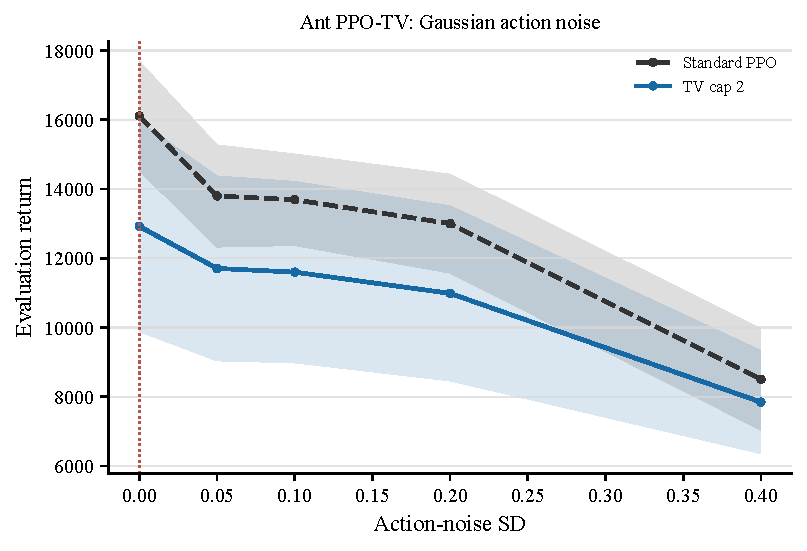
\includegraphics[width=\linewidth]{plots/ant_ppo_tv30/action_noise.pdf}
\caption{Gaussian action noise}
\end{subfigure}\par\medskip
\begin{subfigure}{0.48\textwidth}\centering
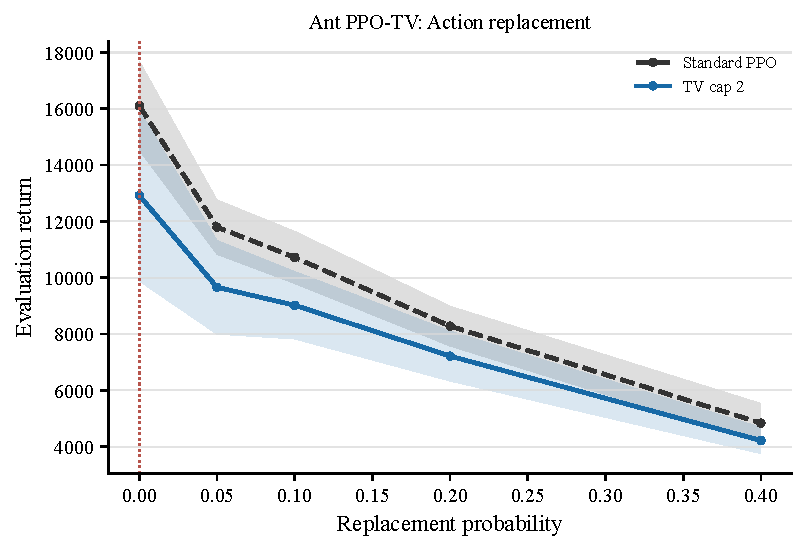
\includegraphics[width=\linewidth]{plots/ant_ppo_tv30/action_replacement.pdf}
\caption{Action replacement}
\end{subfigure}\hfill
\begin{subfigure}{0.48\textwidth}\centering
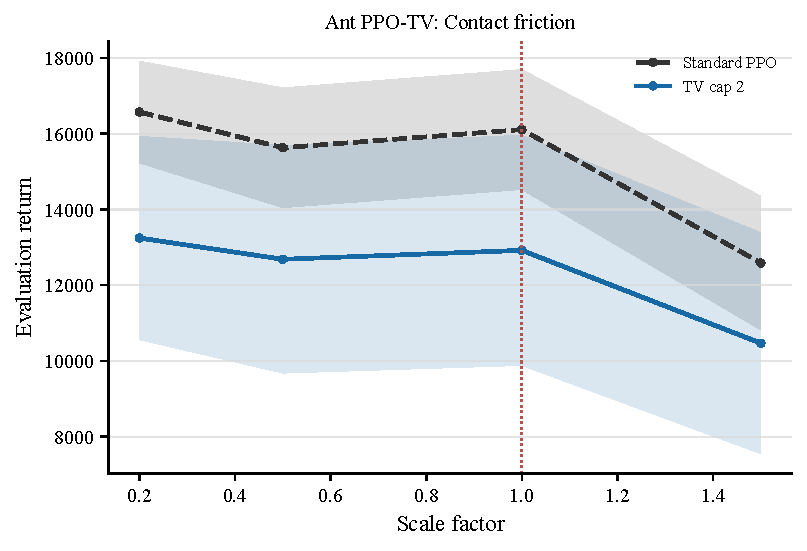
\includegraphics[width=\linewidth]{plots/ant_ppo_tv30/contact_friction.pdf}
\caption{Contact friction}
\end{subfigure}\par\medskip
\caption{Ant PPO-TV. Mean and sample SD across 30 training seeds; ex-post selection.}
\end{figure}
\begin{figure}[p]\centering
\begin{subfigure}{0.48\textwidth}\centering
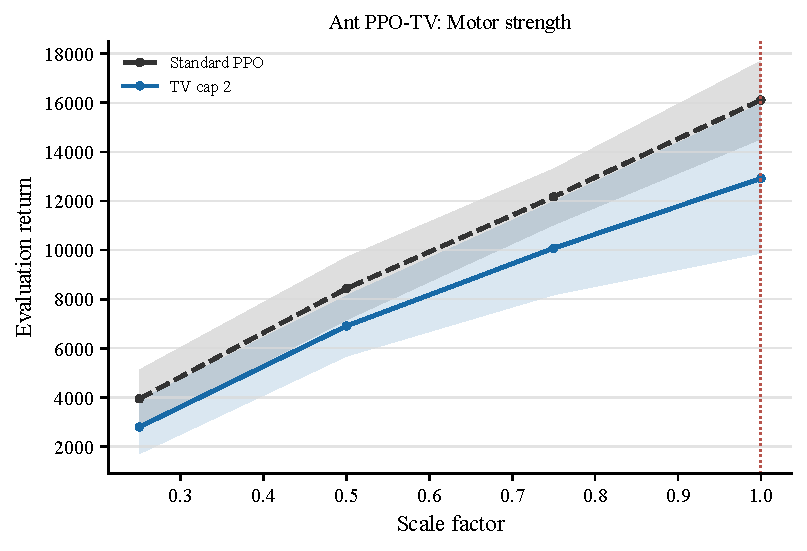
\includegraphics[width=\linewidth]{plots/ant_ppo_tv30/motor_strength.pdf}
\caption{Motor strength}
\end{subfigure}\hfill
\begin{subfigure}{0.48\textwidth}\centering
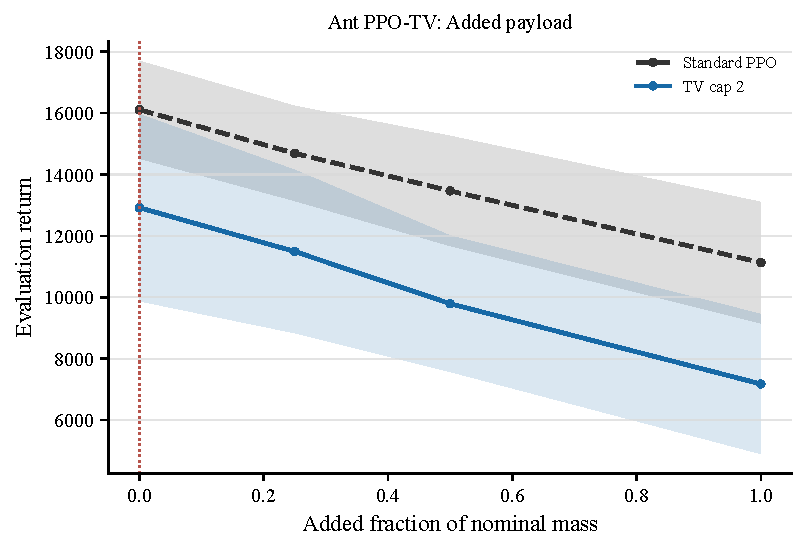
\includegraphics[width=\linewidth]{plots/ant_ppo_tv30/payload_fraction.pdf}
\caption{Added payload}
\end{subfigure}\par\medskip
\caption{Ant PPO-TV. Mean and sample SD across 30 training seeds; ex-post selection.}
\end{figure}
\subsection{Humanoid PPO-TV}
Thirty training seeds per setting. Bands are one sample SD across policy means, not confidence intervals. Ordinary standard is fixed; the best complete parameter is selected ex post separately per axis. 6/6 declared TV caps have full 30-seed suites; 32,768,000 native transitions per policy. Competence not certified by returns/completion.
\begin{figure}[p]\centering
\begin{subfigure}{0.48\textwidth}\centering
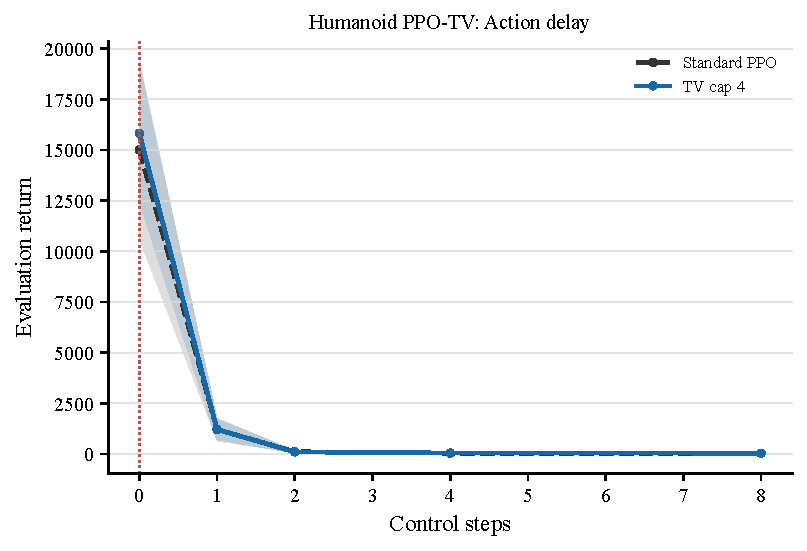
\includegraphics[width=\linewidth]{plots/humanoid_ppo_tv30/action_delay.pdf}
\caption{Action delay}
\end{subfigure}\hfill
\begin{subfigure}{0.48\textwidth}\centering
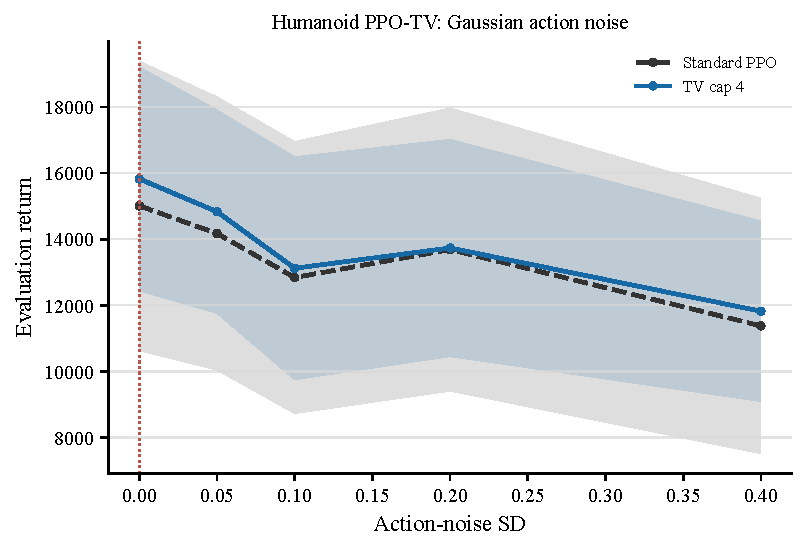
\includegraphics[width=\linewidth]{plots/humanoid_ppo_tv30/action_noise.pdf}
\caption{Gaussian action noise}
\end{subfigure}\par\medskip
\begin{subfigure}{0.48\textwidth}\centering
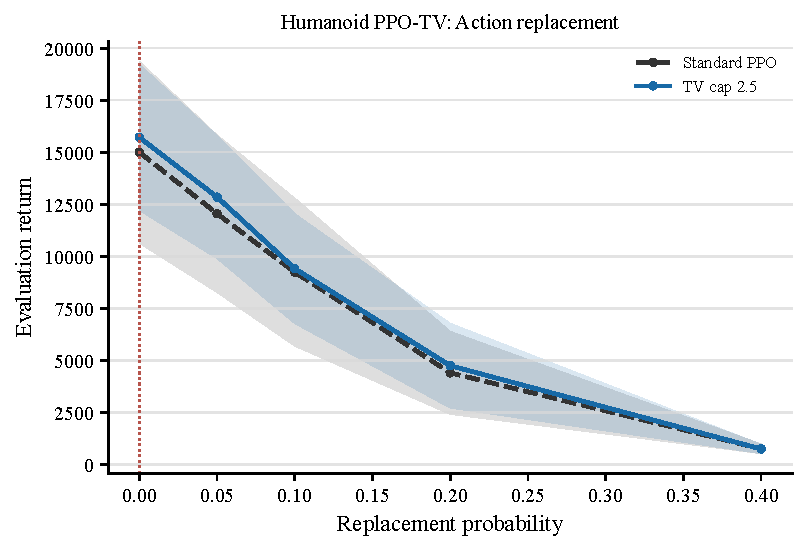
\includegraphics[width=\linewidth]{plots/humanoid_ppo_tv30/action_replacement.pdf}
\caption{Action replacement}
\end{subfigure}\hfill
\begin{subfigure}{0.48\textwidth}\centering
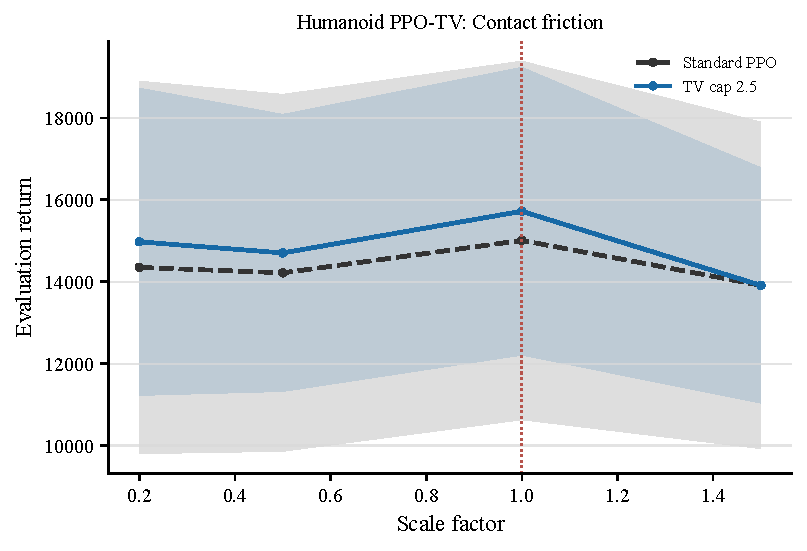
\includegraphics[width=\linewidth]{plots/humanoid_ppo_tv30/contact_friction.pdf}
\caption{Contact friction}
\end{subfigure}\par\medskip
\caption{Humanoid PPO-TV. Mean and sample SD across 30 training seeds; ex-post selection.}
\end{figure}
\begin{figure}[p]\centering
\begin{subfigure}{0.48\textwidth}\centering
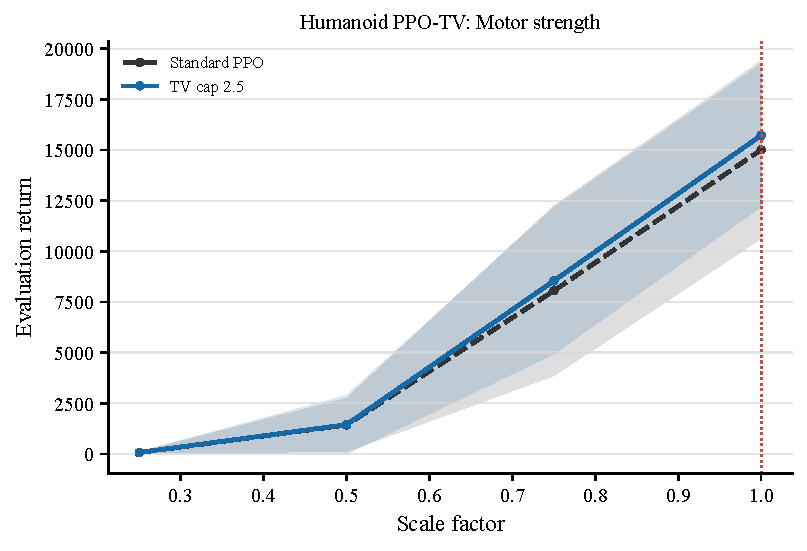
\includegraphics[width=\linewidth]{plots/humanoid_ppo_tv30/motor_strength.pdf}
\caption{Motor strength}
\end{subfigure}\hfill
\begin{subfigure}{0.48\textwidth}\centering
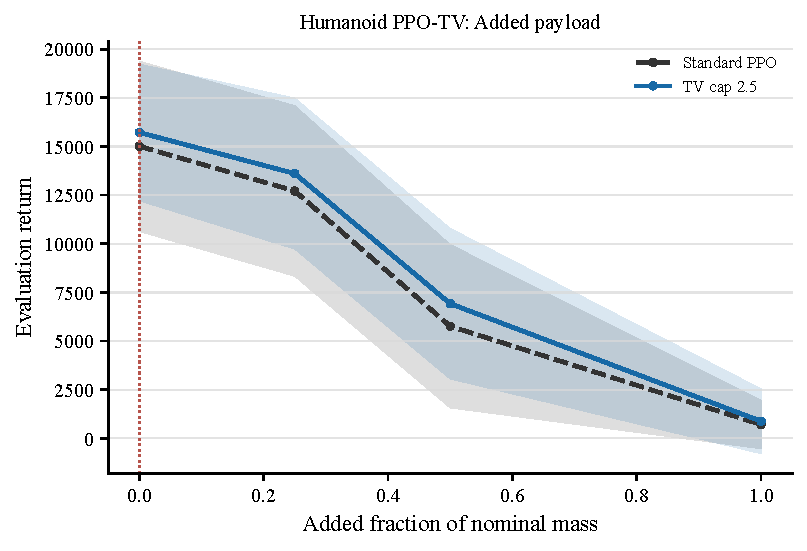
\includegraphics[width=\linewidth]{plots/humanoid_ppo_tv30/payload_fraction.pdf}
\caption{Added payload}
\end{subfigure}\par\medskip
\caption{Humanoid PPO-TV. Mean and sample SD across 30 training seeds; ex-post selection.}
\end{figure}
\subsection{Ant TD3-TV}
Thirty training seeds per setting. Bands are one sample SD across policy means, not confidence intervals. Ordinary standard is fixed; the best complete parameter is selected ex post separately per axis. 6/6 declared TV caps have full 30-seed suites; 512,000 native transitions per policy. Competence not certified by returns/completion.
\begin{figure}[p]\centering
\begin{subfigure}{0.48\textwidth}\centering
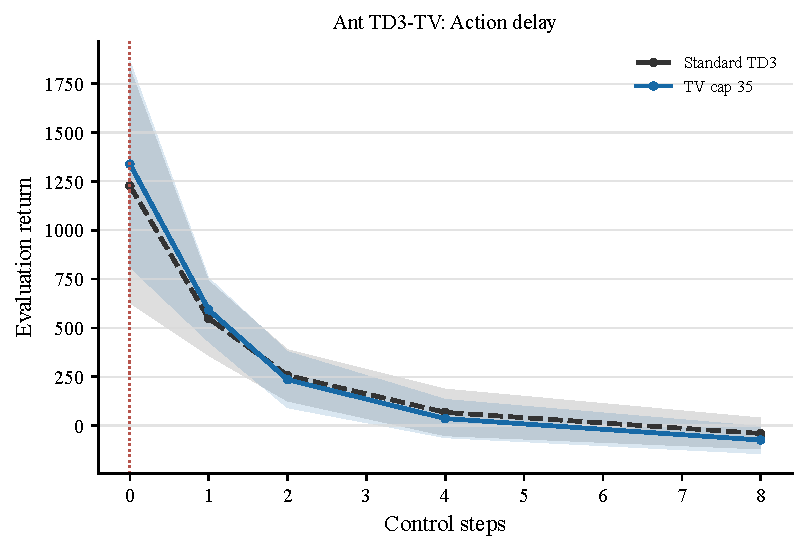
\includegraphics[width=\linewidth]{plots/ant_td3_tv30/action_delay.pdf}
\caption{Action delay}
\end{subfigure}\hfill
\begin{subfigure}{0.48\textwidth}\centering
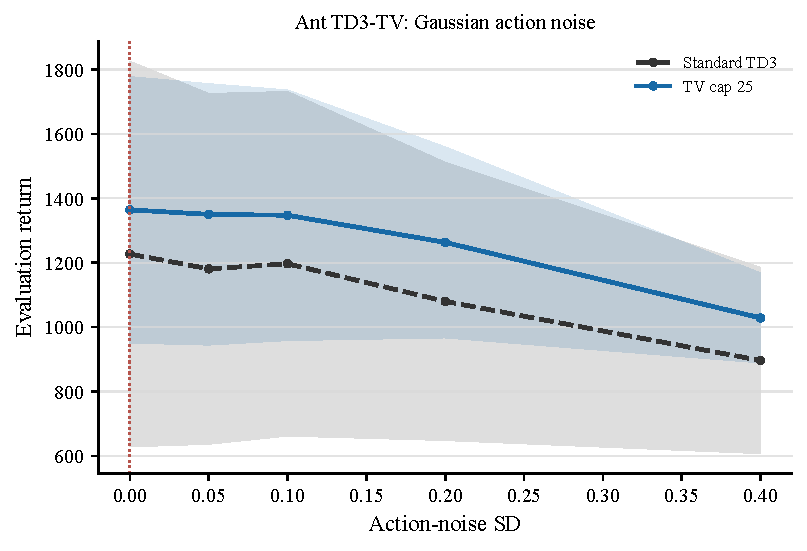
\includegraphics[width=\linewidth]{plots/ant_td3_tv30/action_noise.pdf}
\caption{Gaussian action noise}
\end{subfigure}\par\medskip
\begin{subfigure}{0.48\textwidth}\centering
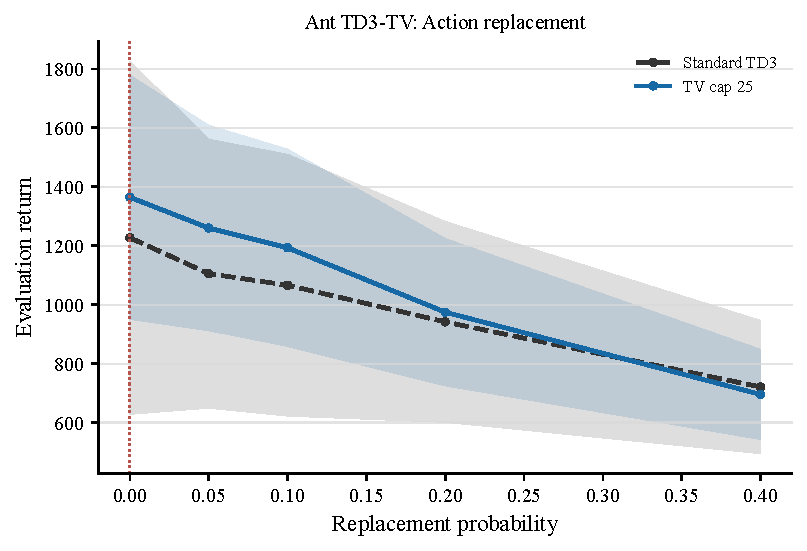
\includegraphics[width=\linewidth]{plots/ant_td3_tv30/action_replacement.pdf}
\caption{Action replacement}
\end{subfigure}\hfill
\begin{subfigure}{0.48\textwidth}\centering
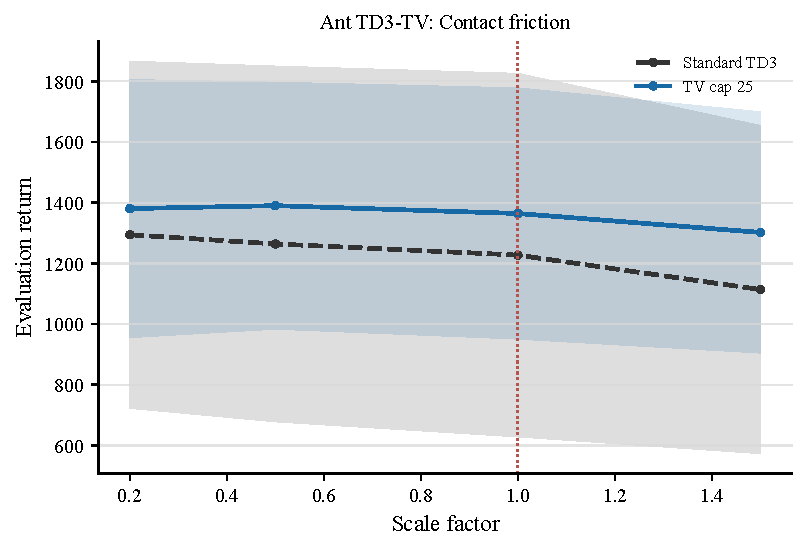
\includegraphics[width=\linewidth]{plots/ant_td3_tv30/contact_friction.pdf}
\caption{Contact friction}
\end{subfigure}\par\medskip
\caption{Ant TD3-TV. Mean and sample SD across 30 training seeds; ex-post selection.}
\end{figure}
\begin{figure}[p]\centering
\begin{subfigure}{0.48\textwidth}\centering
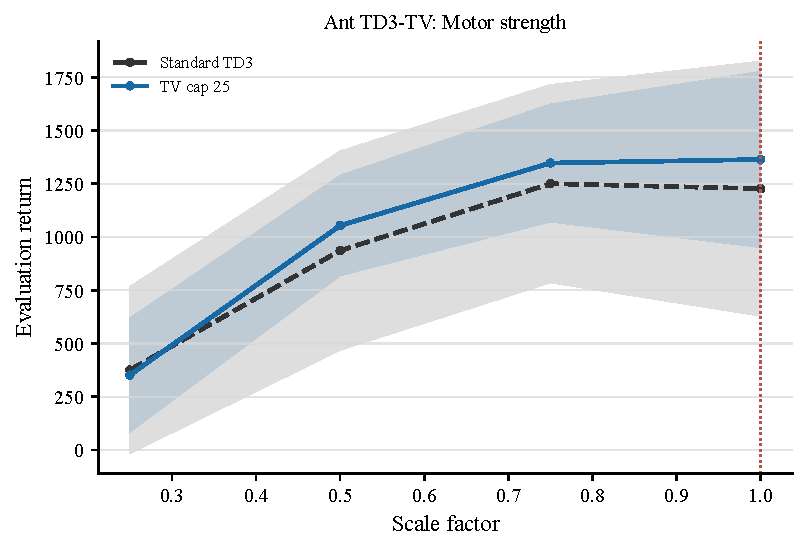
\includegraphics[width=\linewidth]{plots/ant_td3_tv30/motor_strength.pdf}
\caption{Motor strength}
\end{subfigure}\hfill
\begin{subfigure}{0.48\textwidth}\centering
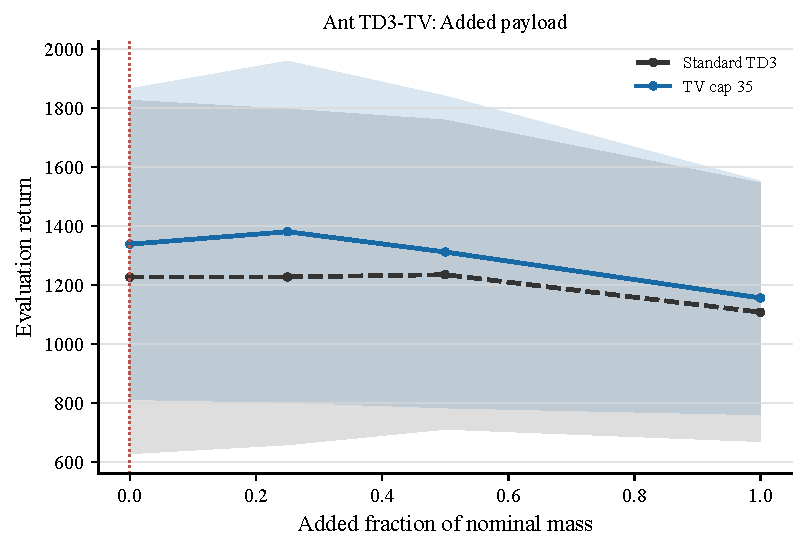
\includegraphics[width=\linewidth]{plots/ant_td3_tv30/payload_fraction.pdf}
\caption{Added payload}
\end{subfigure}\par\medskip
\caption{Ant TD3-TV. Mean and sample SD across 30 training seeds; ex-post selection.}
\end{figure}
\subsection{Drawer PPO-TV}
Thirty training seeds per setting. Bands are one sample SD across policy means, not confidence intervals. Ordinary standard is fixed; the best complete parameter is selected ex post separately per axis. 6/6 declared TV caps have full 30-seed suites; 10,240,000 native transitions per policy. Competence not certified by returns/completion.
\begin{figure}[p]\centering
\begin{subfigure}{0.48\textwidth}\centering
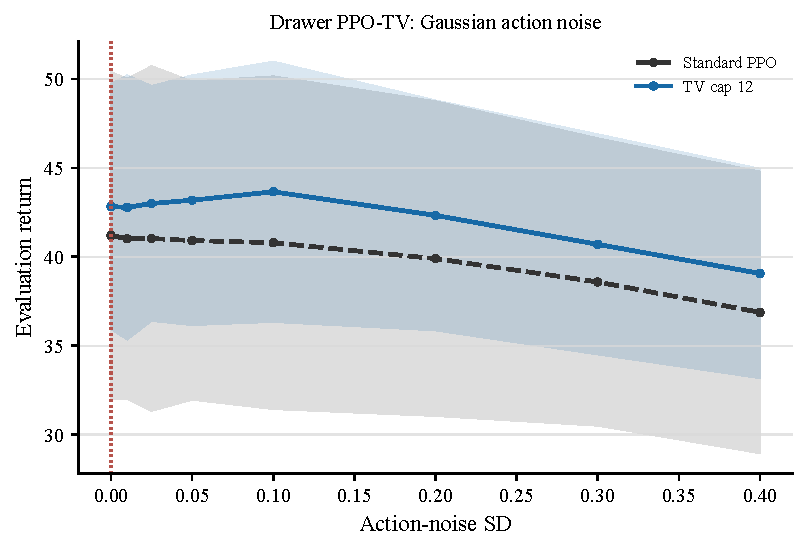
\includegraphics[width=\linewidth]{plots/drawer_ppo_tv30/action_noise.pdf}
\caption{Gaussian action noise}
\end{subfigure}\hfill
\begin{subfigure}{0.48\textwidth}\centering
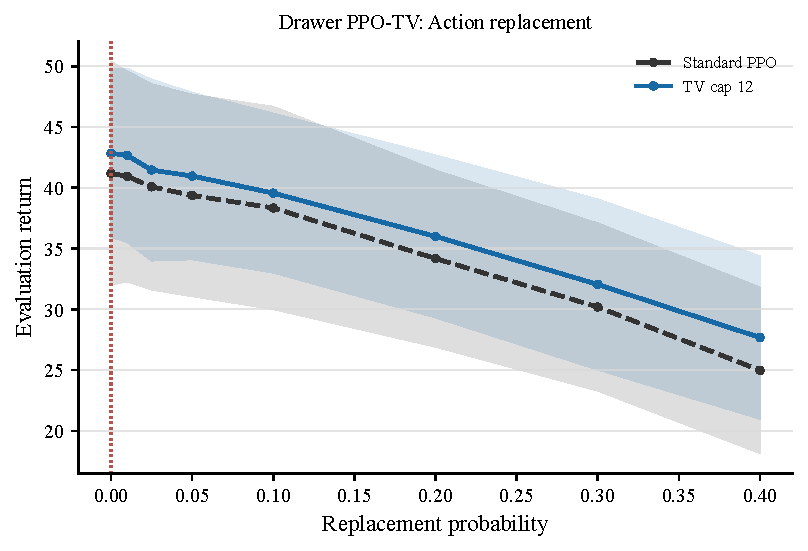
\includegraphics[width=\linewidth]{plots/drawer_ppo_tv30/action_replacement.pdf}
\caption{Action replacement}
\end{subfigure}\par\medskip
\begin{subfigure}{0.48\textwidth}\centering
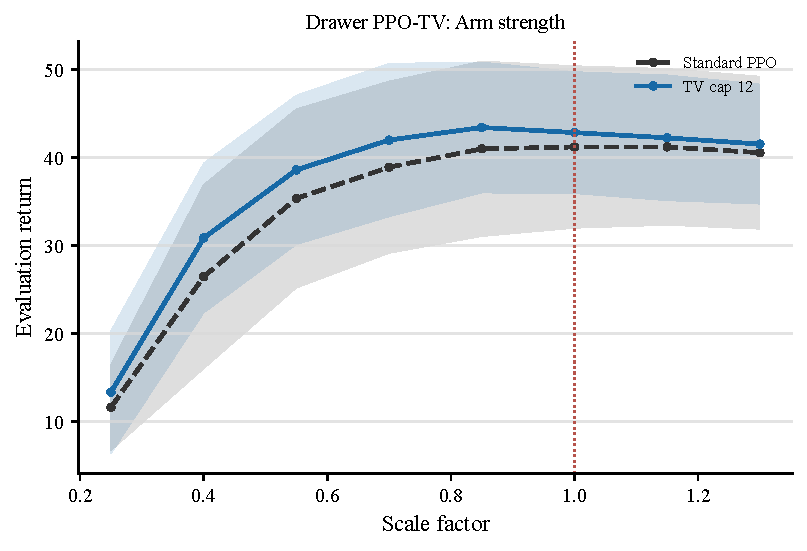
\includegraphics[width=\linewidth]{plots/drawer_ppo_tv30/arm_strength.pdf}
\caption{Arm strength}
\end{subfigure}\hfill
\begin{subfigure}{0.48\textwidth}\centering
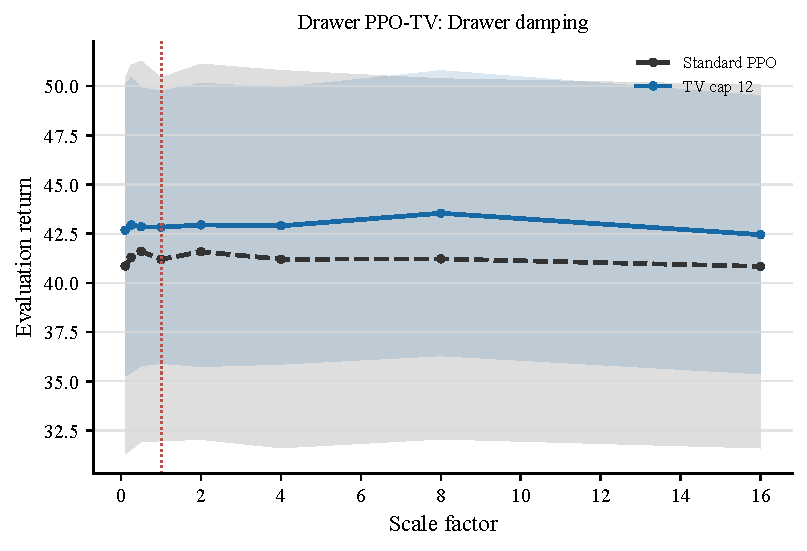
\includegraphics[width=\linewidth]{plots/drawer_ppo_tv30/drawer_damping.pdf}
\caption{Drawer damping}
\end{subfigure}\par\medskip
\caption{Drawer PPO-TV. Mean and sample SD across 30 training seeds; ex-post selection.}
\end{figure}
\begin{figure}[p]\centering
\begin{subfigure}{0.48\textwidth}\centering
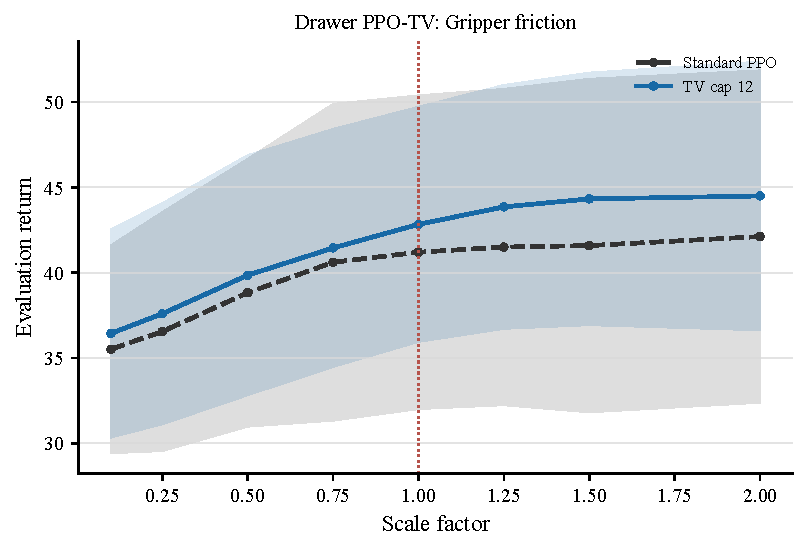
\includegraphics[width=\linewidth]{plots/drawer_ppo_tv30/gripper_friction.pdf}
\caption{Gripper friction}
\end{subfigure}\hfill
\begin{subfigure}{0.48\textwidth}\centering
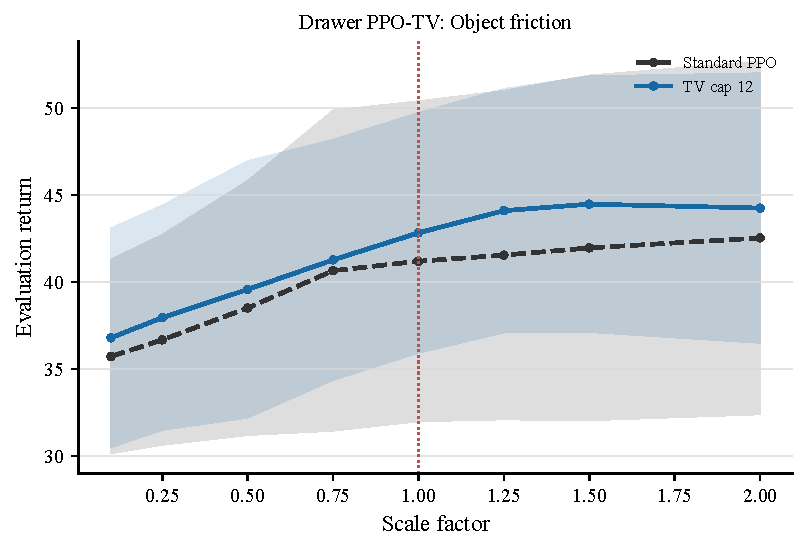
\includegraphics[width=\linewidth]{plots/drawer_ppo_tv30/object_friction.pdf}
\caption{Object friction}
\end{subfigure}\par\medskip
\begin{subfigure}{0.48\textwidth}\centering
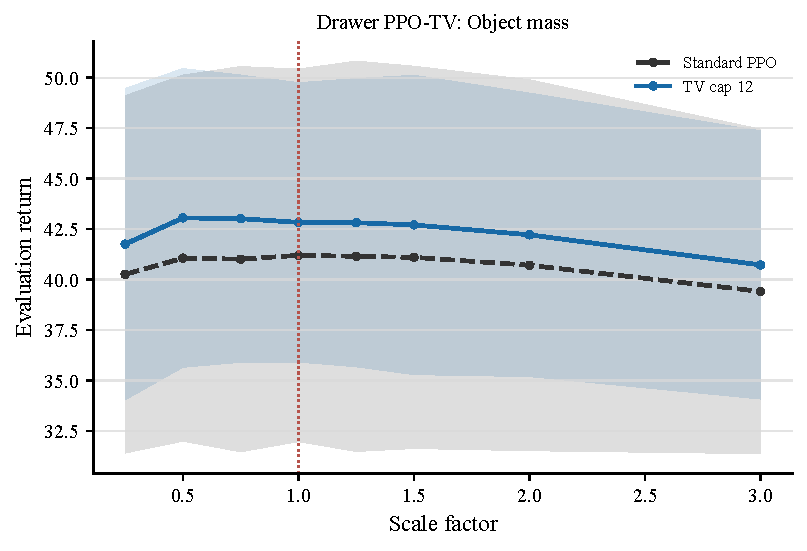
\includegraphics[width=\linewidth]{plots/drawer_ppo_tv30/object_mass.pdf}
\caption{Object mass}
\end{subfigure}\hfill
\caption{Drawer PPO-TV. Mean and sample SD across 30 training seeds; ex-post selection.}
\end{figure}
